\documentclass{article}
\usepackage{float}
\usepackage{hyperref}
\usepackage{url}
\usepackage{graphicx} % Required for inserting images
\usepackage{caption}
\usepackage{subcaption}

\title{Breast cancer risk assessment using Bayesian Networks}
\author{Joachim Verschelde}
\date{May 2024}

\setlength{\textfloatsep}{10pt plus 1.0pt minus 2.0pt}
\setlength{\intextsep}{10pt plus 1.0pt minus 2.0pt}
\setlength{\floatsep}{10pt plus 1.0pt minus 2.0pt}

\begin{document}
\maketitle

\section{Problem domain}
% explanation of the domain of the problem, and of the question that you wish to pose
Megan and her colleague Denise have scheduled an preventive screening examination in their local hospital to check if they have an increased chance of developing breast cancer. 
Because the hospital is short staffed and the waiting list for a mammography or a biopsy is long, they have decided to use a Bayesian Network to help them determine which patients are at an increased risk of developing breast cancer.
The hospital will ask questions or perform tests to determine if the patients have an increased risk, if so a mammography or biopsy is necessary to confirm the presence of cancer.
To build this Bayesian network, the hospital has a database of patients that have been diagnosed with breast cancer in the past, and they used this data to build the Bayesian Network. 
The question for this project is if Megan and Denise are at risk of developing breast cancer.
\section{Network topology}
% - description of the data you used. In particular, for each variable provide: name, type (continue, ordinal, categoric), number of possible values (for discrete variables), or interval of values (for continue variables);
% - figure containing the Bayesian Network;
% - description of the process you followed in order to produce the Bayesian Network. How did you select those variables? How did you determine the relations between them? Did you do something to limit the complexity of the network?;

\begin{figure}[H]
    \centering
    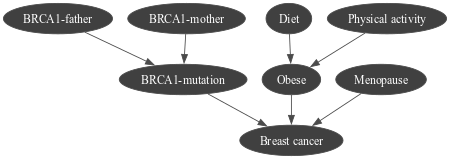
\includegraphics[width=\textwidth]{../figures/network.png}
    \caption{Bayesian Network for Breast Cancer Risk Assessment}
    \label{fig:bayesian_network}
\end{figure}

\begin{table}[H]
    \centering
    \caption{Variable Description}
    \label{tab:variables}
    \begin{tabular}{|c|c|c|}
        \hline
        \textbf{Name} & \textbf{Type} & \textbf{Domain} \\
        \hline
        Breast cancer & Categoric & \{Yes, No\} \\
        Menopause & Categoric & \{Before, After\} \\
        Obese & Categoric & \{No, Moderate, Severe\} \\
        Diet & Categoric & \{Unhealthy, Normal, Healthy\} \\
        Physical activity & Categoric & \{None, Little, Regular\} \\
        BRCA1-mutation & Categoric & \{Yes, No\} \\
        BRCA1-father & Categoric & \{Yes, No\} \\
        BRCA1-mother & Categoric & \{Yes, No\} \\
        \hline
    \end{tabular}
\end{table}

The selection of variables for the Bayesian Network was based on their known or potential impact on breast cancer risk \cite{cancergov} \cite{komen}. The primary variables include genetic factors,
 lifestyle choices, and menopause. Furthermore we discretized the variables to make the network easier to interpret and to reduce the complexity of the network. For example in stead of the variable "Age" we used the variable "Menopause" which is a categoric variable with only 2 values "Before" and "After" indicating if the patient has already reached menopause.

\begin{itemize}
    \item \textbf{Breast cancer}: The target variable representing the presence or absence of breast cancer.
    \item \textbf{BRCA1-mutation}: A mutation in the BRCA1 gene that is strongly associated with an increased risk of breast cancer.
    \item \textbf{BRCA1-father} and \textbf{BRCA1-mother}: indicates whether a parent carries the BRCA1 mutation, affecting the likelihood of the offspring having the mutation.
    \item \textbf{Obese}: Obesity is a well-documented risk factor for breast cancer \cite{komen}.
    \item \textbf{Physical activity}: Regular physical activity burns calories and therefor reduces the chance of becoming obese.
    \item \textbf{Diet}: People who eat a healthy diet are less likely to become obese.
    \item \textbf{Menopause}: The menopause affects hormone levels, which in turn influence breast cancer risk. \cite{surakasula2014comparative}
\end{itemize}
\subsection{Causal and associative relations}
\subsubsection{Breast Cancer 1 (BRCA1) gene mutation}
There is a causal relation between the BRCA1-father/mother variables and the BRCA1-mutation variable, as you inherit the genes of you parents, and if one of you're parents has a BRCA1 gene mutation the odds are 50\% that you will also inherit this mutation \cite{cancergov}.
\subsubsection{The influence of diet and physical activity on obesity} 
There is also a causal relation between the physical activity and the obese variable. Regular physical activity burns calories and helps to maintain a healthy weight and reduce obesity, whereas a lack of physical activity, can lead to weight gain and obesity.
  Therefore, changes in physical activity levels directly affect the likelihood of becoming obese. Furthermore there is also a causal relation between the diet 
  and the obese variable because people that are on a healthy diet eat less calorie-dense foods or are often in a caloric deficit which again directly controls the likelihood of becoming obese.
\subsubsection{What causes breast cancer?}
There is an associative relation between the menopause and presence of breast cancer, this is because the menopause does not directly increase the risk of breast cancer, but aging factors and the hormonal changes that occur during the menopause do.
A mutation in the BRCA1 gene however could cause breast cancer, as the BRCA1 gene helps repair damaged DNA. When the BRCA1 gene is mutated, DNA damage may not be repaired properly and this could lead to breast cancer \cite{brca1}.
It is difficult to tell if obesity causes breast cancer, but there is definitely an association between obesity and breast cancer, especially when the patient has reached menopause \cite{agurs2019many}.

\section{Implementation using Pyagrum}
% description of how you implemented the network using pyAgrum: which functions did you use, and why?;
The code for the experiments can be found on the following GitHub repository: \url{https://github.com/JoachimVerscheldePersonal/BRAL_Assignment1}.
I used the fastBN function to create the Bayesian Network, because it is a fast and natural way to declare the variables, their possible values and the relations between them.
\begin{figure}[H]
    \centering
    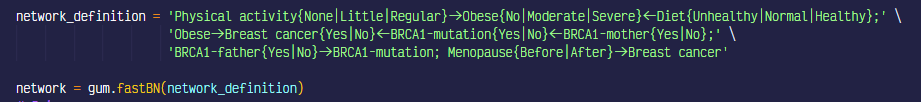
\includegraphics[width=\textwidth]{../figures/network_definition.png}
    \caption{network definition using pyAgrum}
    \label{fig:bayesian_network}
\end{figure}

The prior probabilities for the root nodes are defined using the cpt function. However there are multiple ways to use the cpt function, in my opinion the dictionary method is the most readable.
I tried to underpin these prior probabilities with data found online. (BRCA1-father, BRCA1-mother \cite{cancergov}, Physical activity \cite{eucommission}, Diet \cite{eurostat2}, Menopause \cite{ourworldindata})

\begin{figure}[H]
    \centering
    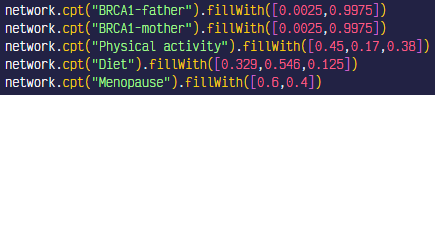
\includegraphics[width=\textwidth]{../figures/prior_declaration.png}
    \caption{Declaration of the properly probabilities using pyAgrum}
    \label{fig:prior_declaration}
\end{figure}
To define the conditional probability tables, I again used the dictionary method as this again was the most readable in my opinion.

\begin{figure}[H]
    \centering
    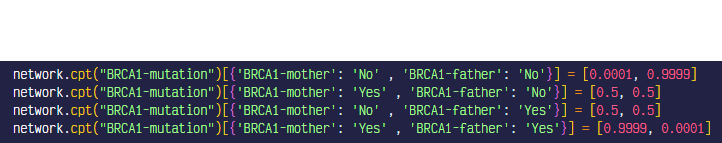
\includegraphics[width=\textwidth]{../figures/cpt_declaration.png}
    \caption{Example of a conditional probability table declaration using pyAgrum}
    \label{fig:cpt_declaration}
\end{figure}

%TODO SET EVIDENCE AND CAUSAL NETWORK showCausalImpact
\section{Results}
% description of the results (e.g., the computed probability).;
The prior probabilities at the start of the preventive screening examination are computed using the pyAgrum.lib.notebook.showInference function.
\begin{figure}[H]
    \centering
    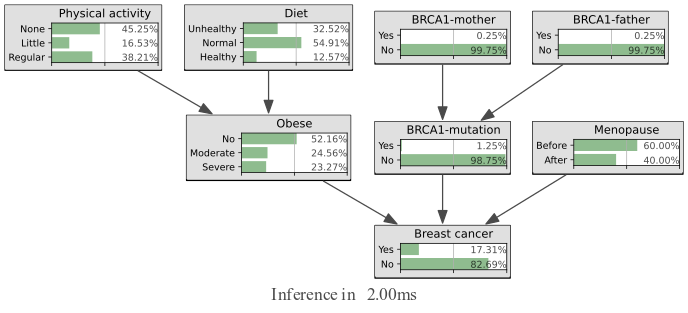
\includegraphics[width=\textwidth]{../figures/priors.png}
    \caption{Prior probabilities}
    \label{fig:priors}
\end{figure}
As can be seen in figure \ref{fig:priors} the prior probability of having breast cancer is $17.31\%$.
\subsection{Family history}
The medical files are checked for a family history of breast cancer, and it is found that the father of Megan has a BRCA1 gene mutation, The parents of Denise do not have a mutation in the BRCA1 gene.
We update the network with this information and compute the posterior probabilities. Therefor we use the exact inference method LazyPropagation.
\begin{figure}[H]
    \centering
    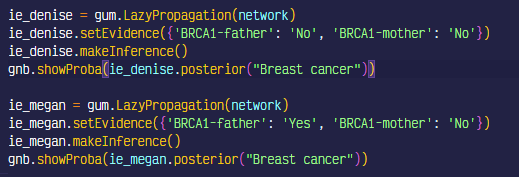
\includegraphics[width=\textwidth]{../figures/inference_BRCA1-parents_code.png}
    \caption{Using the LazyPropagation to compute the posterior probabilities}
    \label{fig:posterior}
\end{figure}

If we set the evidence for Megan and Denise, we see that given the fact that Megan's father has a BRCA1 gene mutation, the probability of Megan having breast cancer increases, while the probability of Denise having breast cancer decreases.


\begin{figure}[H]
    \centering
    \begin{subfigure}{.5\textwidth}
      \centering
      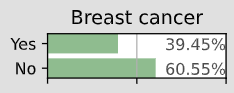
\includegraphics[width=.5\linewidth]{../figures/inference_megan_BRCA1-Father.png}
      \caption{The posterior probabilities for Megan}
      \label{fig:megan_posterior_1}
    \end{subfigure}%
    \begin{subfigure}{.5\textwidth}
      \centering
      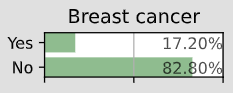
\includegraphics[width=.5\linewidth]{../figures/inference_denice_no_mutation_parents.png}
      \caption{The posterior probabilities for Denise}
      \label{fig:sub2}
    \end{subfigure}
    \label{fig:test}
    \end{figure}

    \subsection{Obesity check using BMI}
    The next step in the screening procedure is a BMI check. The Body Mass Index (BMI) of Megan and Denise is measured and the menopausal status is taken into account. 
    This is done because in the postmenopausal state obesity increases the risk of breast cancer while in premenopausal state, obesity decreases the risk of breast cancer \cite{garcia2021obesity}.
    It is found that Megan has a BMI of 40 and Denise has a BMI of 21. Therefor Denise is moderate obese and Megan is severe obese. 
    Furthermore Denise is 22 years old and in premenopausal state, whilst Megan is 55 years old and is in postmenopausal state.
    We update the network with this information and again compute the posterior probabilities. By setting the obese variable, the ancestors of the obese variable become independent of the breast cancer variable.
    \begin{figure}[H]
        \centering
        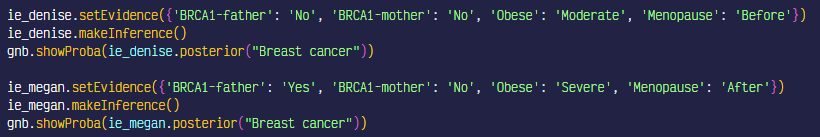
\includegraphics[width=\textwidth]{../figures/inference_obese_menopause_code.png}
        \caption{Using the LazyPropagation to compute the posterior probabilities}
        \label{fig:posterior_2}
    \end{figure}

    \begin{figure}[H]
        \centering
        \begin{subfigure}{.5\textwidth}
          \centering
          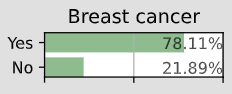
\includegraphics[width=.4\linewidth]{../figures/inference_obese_menopause_megan.png}
          \caption{The posterior probabilities for Megan}
          \label{fig:megan_posterior_2}
        \end{subfigure}%
        \begin{subfigure}{.5\textwidth}
          \centering
          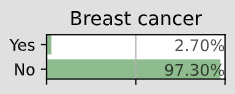
\includegraphics[width=.4\linewidth]{../figures/inference_obese_menopause_denise.png}
          \caption{The posterior probabilities for Denise}
          \label{fig:Denise_posterior_2}
        \end{subfigure}
        \label{fig:test}
        \end{figure}
\section{Screening result and recommendations}
Given the evidence from the family history and the BMI check, Denise has a $2.7\%$ chance of developing breast cancer and therefor can go home immediately.
Megan on the other hand has a $78.11\%$ chance of developing breast cancer and therefor needs further examination.
Fortunately the result of Megan's mammography is negative, and therefor Megan can also go home.
However the doctors have some recommendations for Megan. Using the Bayesian network to compute what the probability of breast cancer would be if Megan would exercise more regularly and eat healthy, the probability of developing breast cancer could decrease to $41.15\%$.

\begin{figure}[H]
    \centering
    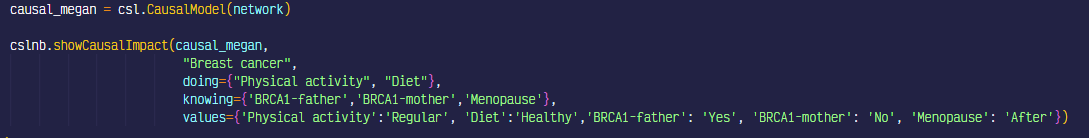
\includegraphics[width=\textwidth]{../figures/causal_megan_code.png}
    \caption{Using the causal model to compute impact of diet and physical activity on breast cancer risk}
    \label{fig:causal:1}
\end{figure}



\section{Discussion and conclusions}
% discussion and conclusions, where you also reflect on the result you obtained.
% Were you successful in finding the answer(s) to your question? What could you have done better?;
The use of a Bayesian Network to identify proved to be effective in determine which patients are at an increased risk of developing breast cancer.
We were able to accurately predict the risk of developing breast cancer for Megan and Denise based on their family history and lifestyle factors.
We showed that Megan has a high risk of developing breast cancer, while Denise has a low risk. Furthermore we showed that by exercising more regularly and eating healthy, the risk of developing breast cancer for Megan could decrease considerably.
Reflecting on the results, we think it was difficult to estimate the prior and conditional probabilities. Because we were not able to learn the probability distributions. 
All in all it was a fun and educational project, and it showed how Bayesian networks can be used in practice.
\section{References}
\bibliographystyle{plain}
\bibliography{references}

\end{document}